\chapter{Auswertung, Fehlerrechnung und Diskussion der Messergebnisse}
\section{Aufgabe 1: Einführung}
Um mit dem Versuchsaufbau vertraut zu werden, wird ein Restgasspektrum Massenbereich \SIrange{1}{51}{amu} unter Standardbedingungen ($E = \SI{65}{eV},I_e =\SI{1}{mA}$) aufgenommen. Ein breiteres Spektrum, wie in der Aufgabe gefordert wird hier nicht betrachtet, da nicht zu erwarten ist das die analysierte Raumluft Moleküle mit $\frac{m}{q} > \SI{51}{\frac{amu}{e}}$ enthält. Das gemessene Spektrum ist  
in Abbildung \ref{fig:MSbreitspektrum} zu sehen, zudem sind die durch einen Savitzky-Golay-Filter geglätteten Daten und die erwarteten Peaks eingetragen. Es ist sichtbar, dass das gemessene Spektrum den Erwartungen entspricht, bis auf den hohen Peak im Bereich von Wasserstoff. Aus Laborerfahrung mit RGAs ist bekannt, das diese im Bereich um \SI{1}{amu} selten sinnvolle Ergebnisse liefern. Desweiteren werden die Peaks der erwarteten Raumluftkomponenten näher betrachtet, diese sind in den Abbildungen \ref{fig:MSWasserPeak}-\ref{fig:MSCO2Peak} im Anhang zu sehen.  

\begin{figure}[H]
    \centering
    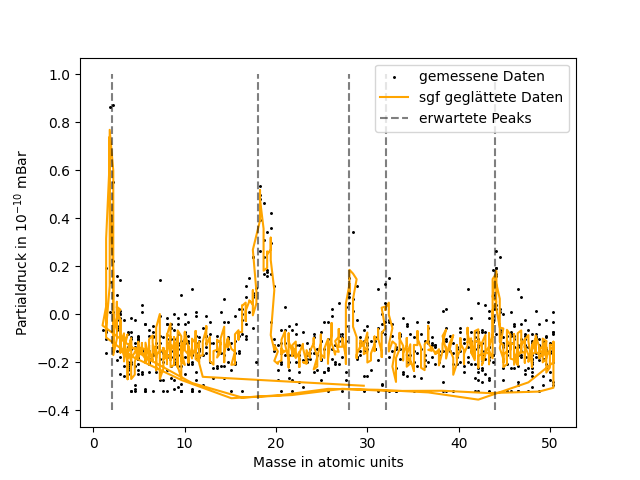
\includegraphics[width=140mm,scale=0.8]{Massenspektrometer/include/MSBreitspektrum.png}
    \caption{Spektrum der Raumluft im Massenbereich \SIrange[]{1}{51}{amu}}
    \label{fig:MSbreitspektrum}
\end{figure}

Der Verlauf des Partialdrucks in Abhängigkeit des Elektronenstroms soll gemessen werden. Dieser ist in Abbildung \ref{fig:MSParDEI} dargestellt. Es ist sichtbar, das der Partialdruck im gemessenen Bereich annähernd linear vom Elektronenstrom abhängt. Die gewählten Standardbedingungen zeigen sich somit als sinnvoll, da sich mit einem maximalem Elektronenstrom von \SI{1}{mA} auch ein maximales Signal bzw. ein maximaler Partialdruck ergibt, was das Signal-Rausch-Verhältnis minimiert. 
\begin{figure}[H]
    \centering
    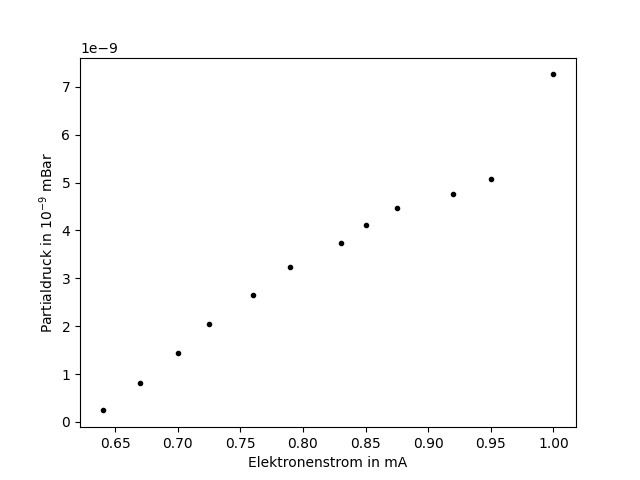
\includegraphics[width=140mm,scale=0.8]{Massenspektrometer/include/MSpardEI.png}
    \caption{Verlauf des Partialdrucks in Abhängigkeit des Elektronenstroms}
    \label{fig:MSParDEI}
\end{figure}

Um das Auflösungsvermögen des Massenspektrometers zu 
berechnen, werden die Peaks aus Abbildungen \ref{fig:MSWasserPeak}-\ref{fig:MSCO2Peak} verwendet. Die Wahl der Definition des Auflösungsvermögen wurde in Kapitel \ref{chapter:MSMassenauflösung} beschrieben. 
Für die gemessenen Peaks ergibt sich somit:

\begin{table}[H]
    \centering
    \caption{Berechnetes Auflösungsvermögen mit $R = \frac{m}{\Delta m}$}
    \begin{tabular}{ccc}
        m in amu & $\Delta$m in amu&  Auflösungsvermögen R\\ \hline
        18.24 & 0.6 &30.4\\
        27.68 & 0.76&36.42\\
        31.36 & 0.76&41.26\\
        43.32 & 1.04&41.65\\\hline
    \end{tabular}
    
    \label{tab:MSAuflösungsvermögen}
\end{table}
In Tabelle \ref{tab:MSAuflösungsvermögen} ist sichtbar, dass das Auflösungsvermögen mit steigender Masse steigt. Dies liegt daran, das die Peakbreite $\Delta m$ unabhängig von der Masse für alle Massen hinreichend konstant ist. 

\section{Aufgabe 2: Auftrittsenergie von Argon}

Zur Berechnung der Auftrittsenergie von Argon, wird pro Ion von Argon ein Partialdruckspektrum in Abhängigkeit der Beschleunigungsspannung bzw. Elektronenenergie aufgenommen. Dabei ergibt sich ab einer bestimmten Auftrittsenergie ein exponetieller Verlauf des Partialdrucks. Um diese Auftrittsenergie zu bestimmen, passen wir eine Gerade der Form: $$p(E) = a\cdot E + b$$ an den annäherend linearen Beginn des exponentiellen Graphen an. Mit den angepassten Parametern lässt sich dann der Schnittpunkt mit der x-Achse bilden: $$E(p=0) = -\frac{b}{a}$$ was der Auftrittsenergie entspricht. Leider ist ein Datensatz dieser Aufgabe verloren worden, sodass nur die Auftrittsenergie des einfach ionisierten Argons bei \SI{40}{amu} bestimmt werden kann. Für zweifach ionisiertes Argon bei \SI{20}{amu} würde die Analyse analog erfolgen. 

In das gemessene Spektrum des einfach ionisierten Argons wird eine Gerade angepasst: 
\begin{figure}[H]
    \centering
    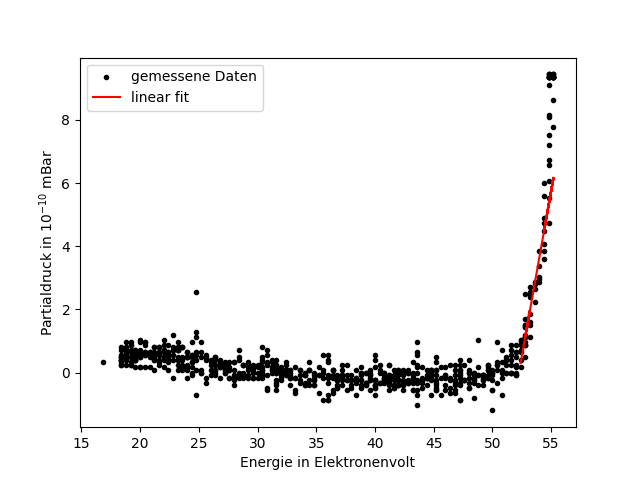
\includegraphics[width=140mm,scale=0.8]{Massenspektrometer/include/MSArgon1Ion.png}
    \caption{Spektrum des Partialdrucks von einfach ionisiertem Argon in Abhängigkeit der Elektronenergie}
    \label{fig:MSArgon1Ion}
\end{figure}
Unter der Annahme von einer Unsicherheit von \SI{5}{\%} auf den Partialdruck ergibt die Anpassung:
$$a = \SI{2.09(2)e-10}{\frac{mBar}{eV}}, b= \SI{-1.09(1)e-8}{mBar}$$
Die Auftrittsenergie ergibt sich somit unter Verwendung von gaußscher Fehlerfortpflanzung zu:
$$E_{aus} = \SI{53.25(0.76)}{eV}$$
Zum Literaturwert, $E_{lit(Ar^+)}= \SI{15.76}{eV}$\cite{VorbereitungsMappe} besteht eine erheblicher Differenz, welche nicht im Fehlerbereich enthalten ist. Vermutlich wurde der falsche Teil des Spektrums an eine Gerade angepasst.   

\section{Aufgabe 3: Dissoziationsenergien von Stickstoff}

Die Dissoziationsenergien von Stickstoff lassen sich unter Kenntnis der Ionisationsenergie $E_I = \SI{14.5}{eV}$ von atomarem Stickstoff aus den Auftrittsenergien berechnen. Zur Berechnung dieser, wird analog zu Aufgabe 2 vorgegangen. Die Spektren und angepassten Geraden sind in den Abbildungen \ref{fig:MSN2Diss} und \ref{fig:MSNDiss} abgebildet.
\begin{figure}[H]
    \centering
    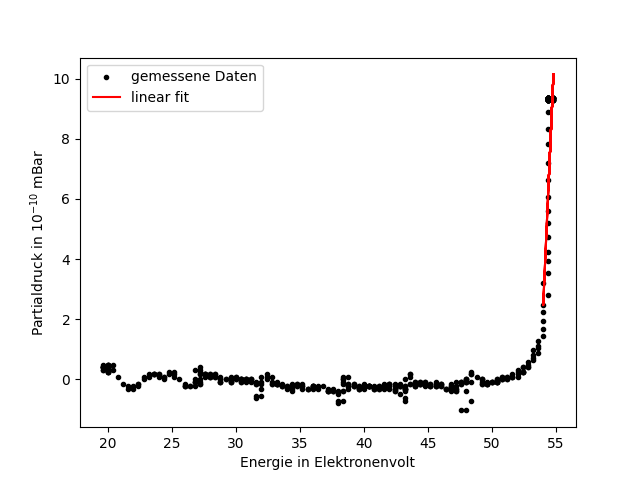
\includegraphics[width=120mm,scale=0.8]{Massenspektrometer/include/MSN2Diss.png}
    \caption{Spektrum des Partialdrucks von einfach ionisiertem molekularem Stickstoff in Abhängigkeit der Elektronenergie}
    \label{fig:MSN2Diss}
\end{figure}
\begin{figure}[H]
    \centering
    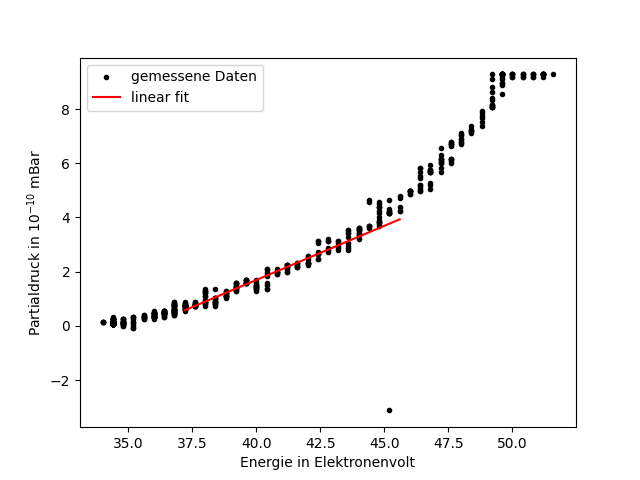
\includegraphics[width=120mm,scale=0.8]{Massenspektrometer/include/MSNDiss.png}
    \caption{Spektrum des Partialdrucks von einfach ionisiertem atomarem Stickstoff in Abhängigkeit der Elektronenergie}
    \label{fig:MSNDiss}
\end{figure}
damit ergibt sich für die Parameter: 
$$a_1 = \SI{ 9.62(0.15)e-10}{\frac{mBar}{eV}}, b_1 = \SI{-5.64(0.08)e-8}{mBar}$$
$$a_2 = \SI{4.09(0.03)e-11}{\frac{mBar}{eV}}, b_2 = \SI{-1.67(0.01)e-9}{mBar}$$
und für die Austrittsenergien: 
$$E_{aus(N_2^+)}= \SI{58.64(1.30)}{eV}$$
$$E_{aus(N^{+})}= \SI{40.03(0.44)}{eV}$$
Die Dissoziationsenergien ergeben sich dann mit
$$E_{D(N_2^+)} = E_{aus(N^+)-E_{aus(N_2^+)}} = \SI{-17.70(1.37)}{eV}$$
$$E_{D(N_2)} = E_{aus(N^+)} - E_I = \SI{26.43(1.30)}{eV}$$
Diese Werte sind offensichtlich unsinnig, lassen sich aber nicht damit erklären das der falsche Bereich des Spektrums linear angepasst wurde. Die genaue Fehlerquelle konnte nicht ausgemacht werden. 

\section{Aufgabe 4: Quantitative Analyse}
Es wird ein weiteres Spektrum von Raumluft aufgenommen und anhand des Cracking-Patterns\cite{VorbereitungsMappe} indiziert. 
Das Spektrum ist in Abbildung \ref{fig:MSzweitesSpektrum} sichtbar. 
Der gemessene Partialdruck aller Peaks ist in Tabelle \ref{tab:MSQuantTable} einsehbar. Da das Massenspektrometer für jede Massenzahl eine andere Sensitivität hat, muss der gemessene Partialdruck um eine die Sensitivität korrigiert werden.
$$p_{korr} = \frac{p}{\sigma}$$
wobei $\sigma$ die Sensitivität ist. 
Die Sensitivitäten für die relevanten Peaks sind gegeben \cite{VorbereitungsMappe}.   

\begin{table}[H]
    \centering
    \caption{Gemessene und korrigierte Partialdrücke und deren Anteil an der Summe der dargestellten Partialdrücke}
    \begin{tabular}{cc|cccc}
        Masse \\in amu & Stoff & $p$ in $10^{-10}$ mBar& Sensitivität& $p_{korr}$ in $10^{-10}$ mBar &Anteil \\\hline
        2& Wasserstoff molekular & 0.24&0.7&0.34&\SI{1.6}{\%}\\
        14& Stickstoff atomar &5.76&1&5.76&\SI{28.4}{\%}\\
        16& Sauerstoff atomar &4.72&0.62&7.6&\SI{37.5}{\%}\\
        18& Wasser &1.52&1.17&1.3&\SI{6.3}{\%}\\
        28& Stickstoff molekular&3.2&1&3.2&\SI{15.8}{\%}\\
        32& Sauerstoff molekular&1.04&0.62&1.7&\SI{8.2}{\%}\\
        40& Argon atomar&0.48&1.16&0.4&\SI{2}{\%}\\
        44& Kohlendioxid&0&0.9&0&\SI{0}{\%}\\\hline
    \end{tabular}
    
    \label{tab:MSQuantTable}
\end{table}

Trockene Luft enthält typischerweise Volumenanteile von \SI{72.08}{\%} Stickstoff, \SI{20.95}{\%} Sauerstoff, \SI{0.93}{\%} Argon und andere Spurengase, wie z.B. Kohlendioxid\cite{Luft}. In feuchter Luft sind diese Anteile in Abhängigkeit der Luftfeuchte geringer. Im gemessenen Spektrum scheint der Argonanteil in dieser Größenordnung zu sein, die Anteile von Stickstoff und Sauerstoff allerdings nicht: Der Sauerstoffanteil ist zu hoch, der Stickstoffanteil zu gering. Das Auftreten eines Wasserstoffpeaks deutet daraufhin das Wasser dissoziert ist, wodurch der Sauerstoffanteil steigen würde und dazu im Verhältnis der Stickstoffanteil sinkt. Die Summe der Partialdrücke ist $\SI{2.03e-9}{mBar}$, was nicht dem Kammerdruck von $\SI{5.4e-9}{mBar}$ entspricht. Um diesen zu erreichen, muss über das gesamte Spektrum integriert werden. Die Summe der Partialdrücke liegt bereits in der richtigen Größenordnung. 


\begin{figure}[H]
    \centering
    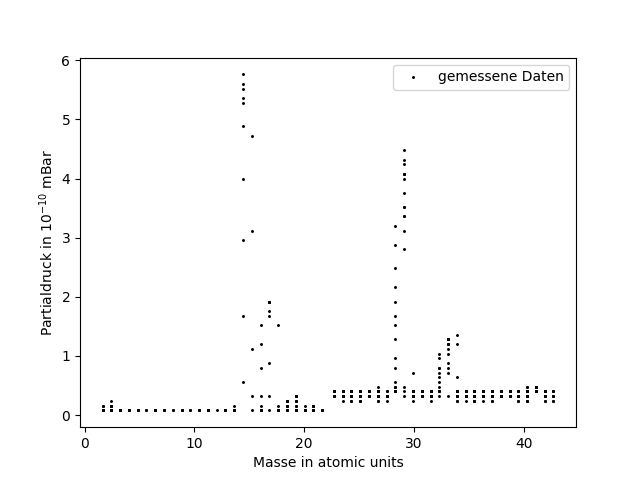
\includegraphics[width=120mm,scale=0.8]{Massenspektrometer/include/MSzweitesSpektrum.png}
    \caption{Spektrum der Raumluft}
    \label{fig:MSzweitesSpektrum}
\end{figure}

\section{Aufgabe 5: Qualitative Analyse}
Ein unbekanntes $\text{C}_X\text{H}_Y$ Gas soll mithilfe des Massenspektrometers bestimmt werden. Dafür werden drei verschiedene Spektren bei den Elektronenenergien $E = {20,30,65} $ eV aufgenommen.
Das Spektrum für \SI{65}{eV} ist in Abbildung \ref{fig:MS65eV} zu sehen, die anderen im Anhang in den Abbildungen \ref{fig:MS20eV},\ref{fig:MS30eV}. 

\begin{figure}[H]
    \centering
    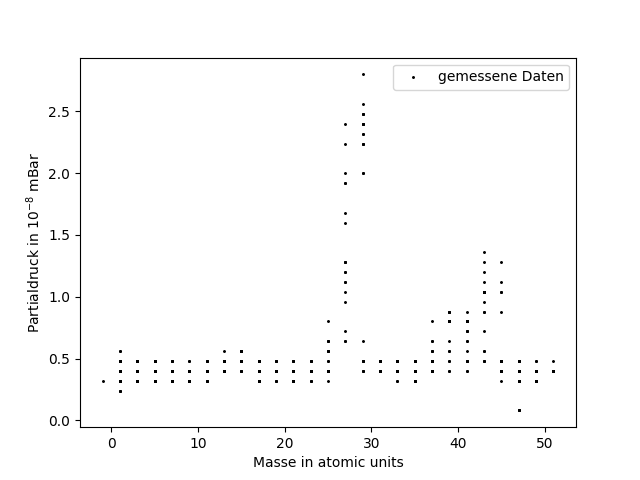
\includegraphics[width=120mm,scale=0.8]{Massenspektrometer/include/MS65eV.png}
    \caption{Spektrum des unbekannten Gases bei einer Elektronenenergie von \SI{65}{eV}}
    \label{fig:MS65eV}
\end{figure}
Ausgehend vom höchsten Peak des \SI{65}{eV}-Spektrums, bei der Masse \SI{29}{amu}, kann man erraten das das unbekannte Gas Propan, also $\text{C}_3
\text{H}_8$ ist. Zur weiteren Analyse wird das \SI{30}{eV}-Spektrum verwendet, da in diesem klare Peaks und eine bessere Messdichte im Vergleich zum \SI{65}{eV}-Spektrum bestehen. In den gemessenen Daten besteht ein negativer Offset, der in Tabelle \ref{tab:MSCracking} korrigiert wird um die erwarteten Peakhöhen zu berechnen. Für einige Massen scheint das erwartete Gas Propan gut zu passen, für die meisten Massen besteht allerdings eine große Abweichung zum erwarteten Wert. Mögliche Fehlerquellen sind zum Beispiel ein ungenügendes Ausspülen von ungewollten Gasen, aber auch die Tatsache das eine TMP schwere Teilchen besser abpumpt als leichtere, wodurch das Ergebnis eventuell verfälscht wird und leichtere Teilchen überproportional vertreten sind. 
\begin{table}[]
    \centering
    \caption{Gemessene und erwartete Peakhöhen für Propan}
    \begin{tabular}{cc|cccc}
        Masse  & gemessene Peakhöhe &gemessene Peakhöhe& erwartete rel.  & erwartete Peakhöhe  \\
        in amu & & +offset & Peakhöhe in \% \\\hline
        12 & -0.22&0.06& 0.4  &0.00608 \\
        13 & -0.24&0.04& 0.5  &0.0076\\
        14 & -0.28&0.& 2.5    &0.038\\
        15 & -0.18&0.1& 3.9   &0.05928 \\
        25 & -0.2 &0.08& 0.7  &0.01064 \\
        26 & -0.12&0.16& 7.6  &0.11552 \\
        27 & 0.14 &0.42& 37.9 &0.57608 \\
        28 & 0.74 &1.02& 59.1 &0.89832 \\
        29 & 1.24 &1.52& 100  &1.52 \\
        30 & 1.06 &1.34& 2.1  &0.03192\\
        36 & -0.2 &0.08& 0.4  &0.00608\\
        37 & -0.18&0.1& 3.1   &0.04712\\
        38 & -0.16&0.12& 4.9  &0.07448\\
        39 & -0.18&0.1& 16.2  &0.24624\\
        40 & -0.04&0.24& 2.8  &0.04256\\
        41 & -0.08&0.2& 12.4  &0.18848\\
        42 & -0.08&0.2& 5.1   &0.07752\\
        43 & 0.02 &0.3& 22.3  &0.33896\\
        44 & 0.22 &0.5& 100   &1.52 \\
        45 & 0.06 &0.34& 1.3  &0.01976 \\
        46 & -0.14&0.14& 0.4  &0.00608 \\\hline
    \end{tabular}
    
    \label{tab:MSCracking}
\end{table}

\section{Aufgabe 6: Thermische Zersetzung}
Der Stoff $\text{CaCO}_3$ wird in der Vakuumkammer bis auf \SI{500}{K} erhitzt. Dabei werden kontinuierlich Spektren von den Massen \SIrange[]{1}{51}{amu} beobachtet. Auffällig ist in diesem vor allem der starke Peak bei \SI{44}{amu}, welche $\text{CO}_2$ entspricht. Dadurch ist zu sehen, das sich beim Erhitzen von $\text{CaCO}_3$ $\text{CO}_2$ abspaltet. Um die Zersetzungsenthalpie $\Delta H$ zubestimmen, wird während des Abkühlungsprozesses der Druck und die Spannung des Thermoelements aufgenommen. Mit der Spannung kann man über eine entsprechende Umrechnungskurve\cite{VorbereitungsMappe} auf die Temperatur schließen. 
Die Zersetzungsenthalpie erhält man aus $$\frac{d \ln{p}}{d T^{-1}} = -\frac{\Delta H}{R} = a\cdot T^{-1}$$ wobei a die Steigung der Gerade ist und $R = \SI{8.314}{\frac{J}{K mol}}$, die sich ergibt wenn $\ln{p}$ über $T^{-1}$ aufgetragen wird. Damit ergibt sich 
$$\Delta H = -a\cdot R$$
Die Messdaten und der lineare Fit sind in Abbildung \ref{fig:MSTherm} aufgetragen. 
Unter einer Annahme einer relativen Unsicherheit von \SI{10}{\%} auf die  Temperatur ergeben sich die Parameter der Anpassung zu
$$a = \SI{-442.14(0.23)}{}$$
$$b = \SI{-15.2232(0.0005)}{}$$

\begin{figure}[H]
    \centering
    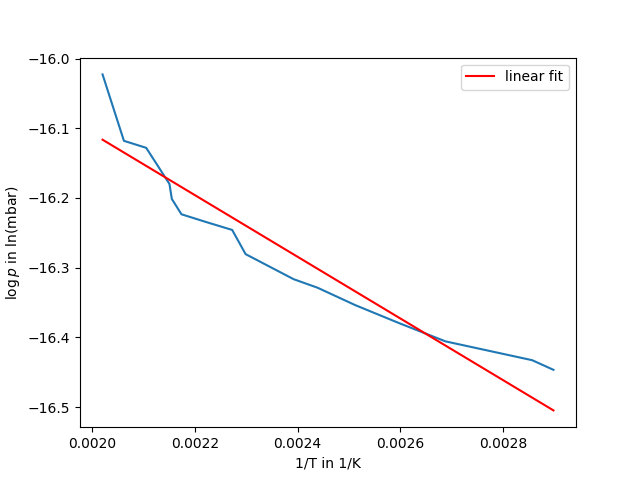
\includegraphics[width=120mm,scale=0.8]{Massenspektrometer/include/MSTherm.png}
    \caption{Messdaten und lineare Anpassung der thermischen Zersetzung}
    \label{fig:MSTherm}
\end{figure}
und somit die Zersetzungsenthalpie zu 
$$\Delta H = \SI{3676(2)}{\frac{kJ}{mol}}$$
Die Standardenthalpie von $\text{CaCO}_3$ ist $\Delta H_{lit} = \SI{-1206.7}{\frac{kJ}{mol}}$\cite{Standardenthalpe}. Ein Vergleich mit diesem Literaturwert ist allerdings nicht sinnvoll, da er unter den Standardbedingungen für Druck und Temperatur ermittelt wurde, was auf dieses Experiment nicht zutrifft. 